\documentclass[11pt]{article}
\usepackage[margin=1in]{geometry}
\usepackage{amsmath,amssymb,amsthm,mathtools}
\usepackage{graphicx,float,microtype}
\usepackage[hidelinks]{hyperref}

\newtheorem{theorem}{Theorem}
\newtheorem{lemma}[theorem]{Lemma}
\newtheorem{corollary}[theorem]{Corollary}
\newcommand{\N}{\mathbb N}
\newcommand{\Z}{\mathbb Z}
\newcommand{\C}{\mathbb C}
\newcommand{\Hh}{\mathbb H_+}
\newcommand{\T}{\mathbb T}
\newcommand{\Om}{\Omega}
\newcommand{\ip}[2]{\left\langle #1,#2\right\rangle}

\title{A two-sided quasihomogeneous zero-product theorem}
\author{Candidate partial result for arXiv:0712.0167}
\date{13 August 2026}

\begin{document}
\maketitle

\noindent\textbf{Status.}
Candidate substantial partial result, likely valid; human review is needed.
The unrestricted Bergman zero-product problem remains open.

\section{Source problem and exact literature boundary}

For a bounded domain $\Om\subset\C^n$, let $P:L^2(\Om)\to A^2(\Om)$
be the Bergman projection and $T_fh=P(fh)$.  Le asks whether
\[
 T_{f_1}\cdots T_{f_N}=0                                  \tag{1.1}
\]
for bounded symbols forces some $f_j=0$ almost everywhere
\cite[Problem~1.1]{Le}.  The source proves this when all but possibly one
symbol are radial on the unit ball, allowing the exceptional $L^2$ symbol to
occur between radial factors.

\begin{figure}[H]
 \centering
 
\includegraphics[width=.82\textwidth]{figures/source_problem_crop.png}
 \caption{Problem~1.1 and its open general Bergman case
 \cite[p.~2]{Le}.}
\end{figure}

The closest later results are precise.  Dong and Zhou prove the two-factor
case when one symbol is arbitrary and the other separately
quasihomogeneous \cite{DongZhou}.  Cuckovic, Huo, and Sahutoglu prove the
zero-product theorem for finite sums of quasihomogeneous symbols on bounded
Reinhardt domains; their Corollary~1 permits one arbitrary symbol at the
\emph{left endpoint} and single-character factors to its right
\cite{CHS}.  The current March 2026 revision still identifies interacting
arbitrary-symbol series as the obstruction.  It does not cover an arbitrary
factor with nontrivial quasihomogeneous strings on both sides.

\begin{figure}[H]
 \centering
 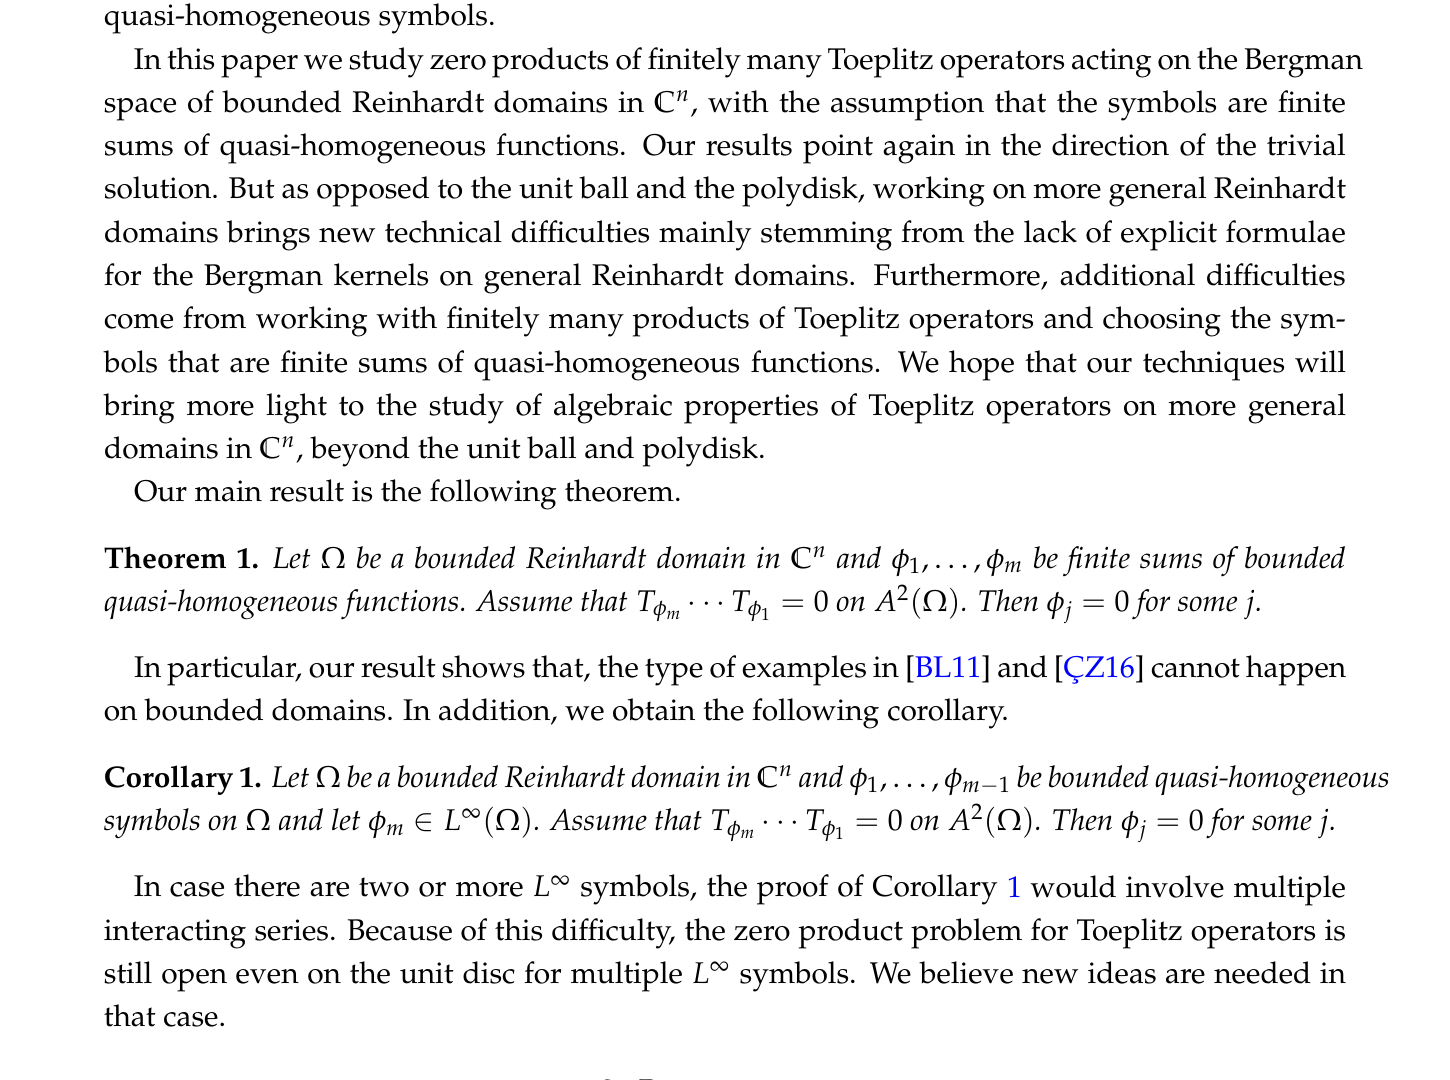
\includegraphics[width=.86\textwidth]{figures/supporting_2026_boundary_crop.png}
 \caption{The closest later theorem, endpoint-arbitrary corollary, and stated
 obstruction in the March 2026 revision of \cite[p.~2]{CHS}.}
\end{figure}

\section{Idea of the proof}

A separately quasihomogeneous Toeplitz operator has exactly one angular
character, so it sends each sufficiently large monomial to one shifted
monomial.  Its scalar weight is a value of a multivariable Mellin transform.
Consequently, a matrix coefficient of a product with one arbitrary middle
symbol is a \emph{scalar product} of a left Mellin factor, one fixed angular
Fourier--Mellin transform of the arbitrary symbol, and a right Mellin factor.

Move the input and output multi-indices together along the positive integer
lattice.  Their angular difference stays fixed, and the scalar product
vanishes at every lattice point.  That lattice is a uniqueness set for
bounded holomorphic functions on a product of right half-planes.  The two
outer factors are nonzero holomorphic functions, so the fixed-frequency
transform of the arbitrary symbol must vanish.  Repeating for every angular
frequency recovers the entire symbol.

The single-character assumption is essential to this proof.  Finite angular
sums on both sides create collisions between different Fourier coefficients
of the middle symbol; two arbitrary symbols create an infinite convolution.

\section{The theorem}

A bounded measurable $a$ on a Reinhardt domain is \emph{separately
quasihomogeneous of degree $p\in\Z^n$} if, away from coordinate hyperplanes,
\[
 a(r_1e^{i\theta_1},\ldots,r_ne^{i\theta_n})
 =A(r_1,\ldots,r_n)e^{i p\cdot\theta}                  \tag{3.1}
\]
for a bounded measurable radial amplitude $A$.

\begin{theorem}\label{thm:main}
Let $\Om\subset\C^n$ be a bounded Reinhardt domain.  Let
$a_1,\ldots,a_r,b_1,\ldots,b_s$ be bounded separately
quasihomogeneous symbols and let $f\in L^2(\Om)$.  If
\[
 T_{a_1}\cdots T_{a_r}\,T_f\,T_{b_1}\cdots T_{b_s}=0 \tag{3.2}
\]
on analytic polynomials, then at least one of
$a_1,\ldots,a_r,f,b_1,\ldots,b_s$ is zero almost everywhere.  Empty left or
right strings are allowed.
\end{theorem}

Thus the exceptional arbitrary symbol may occur at any position.  On the
unit ball, degree-zero separately radial amplitudes already strictly contain
the fully radial class used in the source; arbitrary degrees give weighted
shifts rather than diagonal operators.

\section{Mellin and weighted-shift lemmas}

Write $t_j=|z_j|^2$ and let $E\subset\mathbb R_+^n$ be the radial image of
$\Om$.  A coordinate dilation lets us assume $E\subset[0,1)^n$ without
changing the argument.

\begin{lemma}[integer-lattice uniqueness]\label{lem:lattice}
If $F$ is bounded and holomorphic on $\Hh^n$ and
$F(k)=0$ for every $k\in\N^n$ with all $k_j\ge1$, then $F\equiv0$.
\end{lemma}

\begin{proof}
For one variable, a nonzero bounded holomorphic function on $\Hh$ cannot
vanish at all positive integers: after mapping $\Hh$ to the disk, their
Blaschke sum diverges.  For several variables, fix the last $n-1$ variables
at positive integers and apply the one-variable result in the first
variable.  Then fix an arbitrary first variable and positive integers in the
remaining variables, apply the result in the second variable, and iterate.
\end{proof}

\begin{lemma}[one-character shift]\label{lem:shift}
Let $a$ have degree $p\in\Z^n$ as in (3.1).  For every sufficiently large
$\alpha\in\N^n$,
\[
 T_a z^\alpha=c_a(\alpha)z^{\alpha+p},                \tag{4.1}
\]
where a positive monomial-norm factor times $c_a(\alpha)$ equals
\[
 \mathcal M_a(\alpha)
 :=C_\Om\int_E A(\sqrt t)t^{\alpha+p/2}\,dt.          \tag{4.2}
\]
After translating $\alpha$ by a sufficiently large fixed integer vector,
$\mathcal M_a$ extends to a bounded holomorphic function on $\Hh^n$.  If
$a\ne0$ almost everywhere, that extension is not identically zero.
\end{lemma}

\begin{proof}
Angular orthogonality shows that $P(az^\alpha)$ has only torus character
$\alpha+p$; for large $\alpha$ this character is the monomial
$z^{\alpha+p}$.  Polar integration gives (4.2).  Choose a fixed shift so
every power multiplying $A$ is nonnegative.  The shifted integrand is in
$L^1(E)$, and $|t^u|\le1$ for $u\in\Hh^n$, proving bounded holomorphy by
dominated convergence on compact sub-half-planes.

If the extension were zero, all polynomial moments of the shifted integrand
would vanish.  Extend it by zero from $E$ to $[0,1]^n$.  Stone--Weierstrass
then makes it zero almost everywhere.  The monomial weight is positive off
coordinate hyperplanes, so $A=0$ almost everywhere, a contradiction.
\end{proof}

\section{Proof of Theorem~\ref{thm:main}}

Assume every $a_i$ and $b_j$ is nonzero.  We prove $f=0$.
Iterating Lemma~\ref{lem:shift}, there are total degrees $p,q\in\Z^n$ such
that, for sufficiently large $\beta,\alpha\in\N^n$,
\begin{align}
 T_{a_1}\cdots T_{a_r}z^\beta&=L_0(\beta)z^{\beta+p},\tag{5.1}\\
 T_{b_1}\cdots T_{b_s}z^\alpha&=R_0(\alpha)z^{\alpha+q}.\tag{5.2}
\end{align}
After removing positive monomial-norm factors, $L_0$ and $R_0$ have the
same integer zeros as finite products $L$ and $R$ of fixed translates of
the Mellin transforms (4.2).  Each factor is nonzero by
Lemma~\ref{lem:shift}; hence $L$ and $R$ are nonzero holomorphic functions.

Take the coefficient of $z^{\beta+p}$ in (3.2) applied to $z^\alpha$.
After dividing only the positive norm factors, we obtain
\[
 L(\beta)R(\alpha)
 \int_\Om f(z)z^{\alpha+q}\overline{z^\beta}\,dV(z)=0              \tag{5.3}
\]
for all sufficiently large integer $\alpha,\beta$.

Fix an arbitrary $d\in\Z^n$.  Choose large
$\alpha_0,\beta_0\in\N^n$ so that every intermediate weighted-shift index is
nonnegative and
\[
 \alpha_0+q-\beta_0=d.                                \tag{5.4}
\]
For $u\in\Hh^n$, set
\begin{align}
 B_d(u)&=L(\beta_0+u)R(\alpha_0+u),                   \tag{5.5}\\
 G_d(u)&=\int_\Om f(z)z^{\alpha_0+q}
          \overline{z^{\beta_0}}\prod_{j=1}^n|z_j|^{2u_j}\,dV(z).
                                                                    \tag{5.6}
\end{align}
All fixed powers can be enlarged when choosing $\alpha_0,\beta_0$, so polar
coordinates express $G_d$ as the Mellin transform of an $L^1(E)$ function.
Thus $G_d$ is bounded holomorphic on $\Hh^n$.  The same holds for $B_d$, and
$B_d\not\equiv0$.

Putting $\alpha=\alpha_0+k$ and $\beta=\beta_0+k$ in (5.3) gives
\[
 B_d(k)G_d(k)=0\qquad(k\in\N^n).                      \tag{5.7}
\]
Lemma~\ref{lem:lattice} implies $B_dG_d\equiv0$.  The ring of holomorphic
functions on the connected domain $\Hh^n$ has no zero divisors, and
$B_d\not\equiv0$, so
\[
 G_d\equiv0.                                          \tag{5.8}
\]

For integer $u$, equation (5.6) gives every polynomial moment of the
$(-d)$-th torus Fourier coefficient of $f$, multiplied by the fixed positive
monomial weight from (5.6).  Moment uniqueness on $[0,1]^n$ makes that
coefficient zero almost everywhere on $E$.  Since $d\in\Z^n$ was arbitrary,
all torus Fourier coefficients of $f$ vanish.  Fubini's theorem and Fourier
uniqueness in $L^1(\T^n)$ give $f=0$ almost everywhere, completing the proof.

\section{Consequences and eight upgrade attempts}

\begin{corollary}
On the unit ball, Le's theorem remains true when every radial factor is
replaced by an arbitrary bounded separately quasihomogeneous factor, of any
degree, and the exceptional $L^2$ symbol is placed anywhere in the product.
The same statement holds on every bounded Reinhardt domain.
\end{corollary}

Eight focused routes were audited.  A current-status search confirmed that
the general Bergman problem is still open and separated the 2011 two-factor
and 2020 endpoint results from Theorem~\ref{thm:main}.  Replacing full radial
symmetry by coordinate-torus invariance succeeds through multivariable
Mellin uniqueness.  Allowing nonzero torus degrees succeeds because the
operators remain one-character weighted shifts.  Moving the arbitrary
factor into the interior succeeds by the two-sided matrix coefficient
(5.3).  Passing from the ball to bounded Reinhardt domains succeeds because
only torus orthogonality and moment uniqueness are used.

Three stronger routes fail at a precise point.  Finite character sums on
both sides allow different outer degrees and different Fourier coefficients
of $f$ to collide in one output character, replacing (5.7) by an interacting
sum.  Two arbitrary symbols produce an infinite convolution of two Fourier
series.  Finally, direct cancellation of the outer strings is unavailable:
nonzero quasihomogeneous weighted shifts can have sparse zero weights and
need not be injective or have dense range.  No verified argument removes any
of these obstructions.

Theorem~\ref{thm:main} is therefore a full result for its stated class and a
substantial partial answer to Problem~1.1, not a solution of the unrestricted
problem.

\section{Verification and novelty bounds}

The proof was checked independently at the four sensitive points: all
intermediate exponents can be made nonnegative; positive norm factors are
discarded only on the integer lattice; every shifted outer Mellin transform
is nonzero; and fixed angular difference turns the arbitrary matrix moment
into one Mellin transform.  No computational assertion is used.

The run indexes were searched for arXiv:0712.0167, ``zero-product Toeplitz'',
``separately quasihomogeneous'', ``arbitrary symbol'', and ``Reinhardt''.
Bounded primary-source searches through 13 August 2026 checked Le's source,
Dong--Zhou's 2011 paper, arXiv:2009.01951 in its March 2026 revision, and
recent papers that still describe the arbitrary-symbol Bergman problem as
open.  They found endpoint placement and two-factor results, but no theorem
with quasihomogeneous strings on both sides of an arbitrary factor.  Novelty
confidence is moderate because the literature search was bounded.

Promote for expert review.  The reviewer should focus on the cumulative
degree convention in (5.1)--(5.3) and the standard Laurent-monomial
decomposition on a general Reinhardt domain.

\begin{thebibliography}{9}
\bibitem{Le}
T.~Le,
\emph{The zero-product problem for Toeplitz operators with radial symbols},
arXiv:0712.0167 (2007).

\bibitem{DongZhou}
X.-T.~Dong and Z.-H.~Zhou,
\emph{Algebraic properties of Toeplitz operators with separately
quasihomogeneous symbols on the Bergman space of the unit ball},
J. Operator Theory 66 (2011), 193--207.

\bibitem{CHS}
Z.~Cuckovic, Z.~Huo, and S.~Sahutoglu,
\emph{Zero products of Toeplitz operators on Reinhardt domains},
arXiv:2009.01951, revision of 22 March 2026.
\end{thebibliography}

\end{document}
